\documentclass[journal,12pt,twocolumn]{IEEEtran}

\usepackage{setspace}
\usepackage{gensymb}

\singlespacing


\usepackage[cmex10]{amsmath}

\usepackage{amsthm}

\usepackage{mathrsfs}
\usepackage{txfonts}
\usepackage{stfloats}
\usepackage{bm}
\usepackage{cite}
\usepackage{cases}
\usepackage{subfig}

\usepackage{longtable}
\usepackage{multirow}

\usepackage{enumitem}
\usepackage{mathtools}
\usepackage{steinmetz}
\usepackage{tikz}
\usepackage{circuitikz}
\usepackage{verbatim}
\usepackage{tfrupee}
\usepackage[breaklinks=true]{hyperref}
\usepackage{graphicx}
\usepackage{tkz-euclide}
\usepackage{float}

\usetikzlibrary{calc,math}
\usepackage{listings}
    \usepackage{color}                                            %%
    \usepackage{array}                                            %%
    \usepackage{longtable}                                        %%
    \usepackage{calc}                                             %%
    \usepackage{multirow}                                         %%
    \usepackage{hhline}                                           %%
    \usepackage{ifthen}                                           %%
    \usepackage{lscape}     
\usepackage{multicol}
\usepackage{chngcntr}

\DeclareMathOperator*{\Res}{Res}

\renewcommand\thesection{\arabic{section}}
\renewcommand\thesubsection{\thesection.\arabic{subsection}}
\renewcommand\thesubsubsection{\thesubsection.\arabic{subsubsection}}

\renewcommand\thesectiondis{\arabic{section}}
\renewcommand\thesubsectiondis{\thesectiondis.\arabic{subsection}}
\renewcommand\thesubsubsectiondis{\thesubsectiondis.\arabic{subsubsection}}


\hyphenation{op-tical net-works semi-conduc-tor}
\def\inputGnumericTable{}                                 %%

\lstset{
%language=C,
frame=single, 
breaklines=true,
columns=fullflexible
}
\begin{document}
\newtheorem{theorem}{Theorem}[section]
\newtheorem{problem}{Problem}
\newtheorem{proposition}{Proposition}[section]
\newtheorem{lemma}{Lemma}[section]
\newtheorem{corollary}[theorem]{Corollary}
\newtheorem{example}{Example}[section]
\newtheorem{definition}[problem]{Definition}

\newcommand{\BEQA}{\begin{eqnarray}}
\newcommand{\EEQA}{\end{eqnarray}}
\newcommand{\define}{\stackrel{\triangle}{=}}
\bibliographystyle{IEEEtran}
\providecommand{\mbf}{\mathbf}
\providecommand{\pr}[1]{\ensuremath{\Pr\left(#1\right)}}
\providecommand{\qfunc}[1]{\ensuremath{Q\left(#1\right)}}
\providecommand{\sbrak}[1]{\ensuremath{{}\left[#1\right]}}
\providecommand{\lsbrak}[1]{\ensuremath{{}\left[#1\right.}}
\providecommand{\rsbrak}[1]{\ensuremath{{}\left.#1\right]}}
\providecommand{\brak}[1]{\ensuremath{\left(#1\right)}}
\providecommand{\lbrak}[1]{\ensuremath{\left(#1\right.}}
\providecommand{\rbrak}[1]{\ensuremath{\left.#1\right)}}
\providecommand{\cbrak}[1]{\ensuremath{\left\{#1\right\}}}
\providecommand{\lcbrak}[1]{\ensuremath{\left\{#1\right.}}
\providecommand{\rcbrak}[1]{\ensuremath{\left.#1\right\}}}
\theoremstyle{remark}
\newtheorem{rem}{Remark}
\newcommand{\sgn}{\mathop{\mathrm{sgn}}}
\providecommand{\abs}[1]{\left\vert#1\right\vert}
\providecommand{\res}[1]{\Res\displaylimits_{#1}} 
\providecommand{\norm}[1]{\left\lVert#1\right\rVert}
%\providecommand{\norm}[1]{\lVert#1\rVert}
\providecommand{\mtx}[1]{\mathbf{#1}}
\providecommand{\mean}[1]{E\left[ #1 \right]}
\providecommand{\fourier}{\overset{\mathcal{F}}{ \rightleftharpoons}}
%\providecommand{\hilbert}{\overset{\mathcal{H}}{ \rightleftharpoons}}
\providecommand{\system}{\overset{\mathcal{H}}{ \longleftrightarrow}}
	%\newcommand{\solution}[2]{\textbf{Solution:}{#1}}
\newcommand{\solution}{\noindent \textbf{Solution: }}
\newcommand{\cosec}{\,\text{cosec}\,}
\providecommand{\dec}[2]{\ensuremath{\overset{#1}{\underset{#2}{\gtrless}}}}
\newcommand{\myvec}[1]{\ensuremath{\begin{pmatrix}#1\end{pmatrix}}}
\newcommand{\mydet}[1]{\ensuremath{\begin{vmatrix}#1\end{vmatrix}}}
\numberwithin{equation}{subsection}
\makeatletter
\@addtoreset{figure}{problem}
\makeatother
\let\StandardTheFigure\thefigure
\let\vec\mathbf
\renewcommand{\thefigure}{\theproblem}
\def\putbox#1#2#3{\makebox[0in][l]{\makebox[#1][l]{}\raisebox{\baselineskip}[0in][0in]{\raisebox{#2}[0in][0in]{#3}}}}
     \def\rightbox#1{\makebox[0in][r]{#1}}
     \def\centbox#1{\makebox[0in]{#1}}
     \def\topbox#1{\raisebox{-\baselineskip}[0in][0in]{#1}}
     \def\midbox#1{\raisebox{-0.5\baselineskip}[0in][0in]{#1}}
\vspace{3cm}
\title{ASSIGNMENT 7}
\author{C.RAMYA TULASI}
\maketitle
\newpage
\bigskip
\renewcommand{\thefigure}{\theenumi}
\renewcommand{\thetable}{\theenumi}
Download all python codes from 
\begin{lstlisting}
https://github.com/CRAMYATULASI/ASSIGNMENT7/tree/main/ASSIGNMENT7/CODES
\end{lstlisting}
%
Latex-tikz codes from 
%
\begin{lstlisting}
https://github.com/CRAMYATULASI/ASSIGNMENT7/tree/main/ASSIGNMENT7
\end{lstlisting}
%
\section{Question No 2.79}
Find points on the curve $\vec{x}^T\myvec{\frac{1}{9} & 0 \\ 0 & \frac{1}{16}}\vec{x} = 1$
at which tangents are
\begin{enumerate}
\item  parallel to x-axis
\item  parallel to y-axis.
\end{enumerate}
\section{SOLUTION}
Given curve,
\begin{align}
\vec{x}^T\myvec{\frac{1}{9} & 0 \\ 0 & \frac{1}{16}}\vec{x} = 1 \label{2.0.1}
\end{align}
where,
\begin{align}
\vec{V}&=\myvec{\frac{1}{9} & 0 \\ 0 & \frac{1}{16}},\vec{V}^{-1}=\myvec{9&0\\0&16}\vec{u}=0, \vec{f} = -1 
\end{align}
\begin{align}
|\vec{V}| > 0
\end{align}
$\therefore $ Given curve \eqref{2.0.1} is ellipse.

For an ellipse, point of contact for tangent is
\begin{align}
\vec{q}&=\vec{V}^{-1}(\kappa\vec{n}-\vec{u})\\
&=\vec{V}^{-1}\kappa\vec{n}\quad\quad\quad(\because \vec{u}=0). \label{2.0.5}
\end{align}
where,
\begin{align}
\kappa=&\pm \sqrt{\frac{\vec{u^T}\vec{V}^{-1}\vec{u}-\vec{f}}{\vec{n^T}\vec{V}^{-1}\vec{n}}}\\
      =&\pm \sqrt{\frac{-\vec{f}}{\vec{n^T}\vec{V}^{-1}\vec{n}}}\label{2.0.7}\quad \quad\quad(\because \vec{u}=0)
\end{align}
\begin{enumerate}
\item Tangents are parallel to x-axis then direction and normal vectors are,
\begin{align}
\vec{m_1} = \myvec{1\\0},\vec{n_1} = \myvec{0\\1},
\kappa_1 &=\pm \sqrt{\frac{-\vec{f}}{\vec{n_1^T}\vec{V}^{-1}\vec{n_1}}} \\
 &=\pm\frac{1}{4}
\end{align}
$\therefore$ By Substituting $\kappa_1,\vec{n_1},\vec{V}^{-1}$ in \eqref{2.0.5}
\begin{align}
\vec{q}&=\vec{V}^{-1}\kappa_1\vec{n_1} \\
&=\myvec{0\\\pm4}
\end{align}
$\therefore$ Point of contact for tangents of ellipse are,
\begin{align}
  \vec{q_1}=\myvec{0\\4},\vec{q_2}=\myvec{0\\-4}
\end{align}
\item Tangents are parallel to y-axis then direction and normal vectors are,
\begin{align}
\vec{m_2} = \myvec{0\\1},\vec{n_2} = \myvec{1\\0},
\kappa_2 &=\pm \sqrt{\frac{-\vec{f}}{\vec{n_2^T}\vec{V}^{-1}\vec{n_2}}} \\
 &=\pm\frac{1}{3}
\end{align}
$\therefore$ By Substituting $\kappa_2,\vec{n_2},\vec{V}^{-1}$ in \eqref{2.0.5}
\begin{align}
\vec{q}&=\vec{V}^{-1}\kappa_2\vec{n_2} \\
&=\myvec{0\\\pm3}
\end{align}
$\therefore$ Point of contact for tangents of ellipse are,
\begin{align}
  \vec{q_3}=\myvec{3\\0},\vec{q_4}=\myvec{-3\\0}
\end{align}
\end{enumerate}

Plot of Tangents to the given curve -
\numberwithin{figure}{section}
\begin{figure}[!ht]
    \centering
    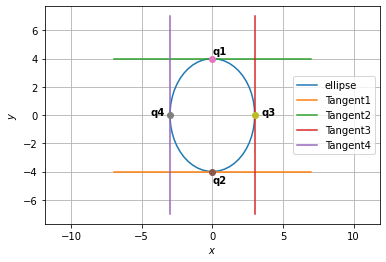
\includegraphics[width=\columnwidth]{ELLIPSE.png}
    \caption{Tangents to ELLIPSE.}
    \label{fig:Tangent to ELLIPSE.}
\end{figure}  
\end{document}
